\documentclass{article}

\usepackage[utf8]{inputenc}
\usepackage[spanish]{babel}
\usepackage{amsthm}
\usepackage{nccmath}
\usepackage{enumitem}
\usepackage{graphicx}
\usepackage{verbatim}
\usepackage{algpseudocode}

\theoremstyle{plain}
\newtheorem{proposicion}{Proposición}

\theoremstyle{definition}
\newtheorem{definition}{Definición}[section]
\newtheorem{example}{Ejemplo}[section]

\title{Teoría de Autómatas y Lenguajes Formales\\[.4\baselineskip]Práctica 3.}
\author{Alejandro Rodríguez Moreno}
\date{Diciembre 2022}

\begin{document}

\maketitle

\section{Define the TM solution of exercise 3.4 of the problem list and test its correct behaviour. }

\begin{center} 
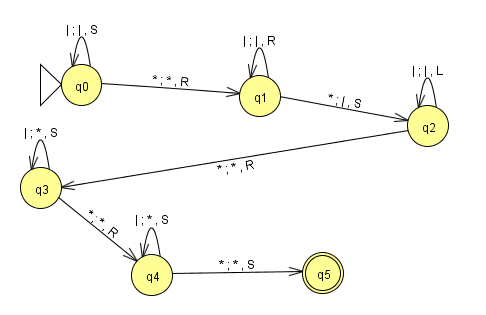
\includegraphics[width=10cm, height=7cm]{P3_E1.png}
\end{center}
\section {Define a recursive function for the sum of three values.}

\begin{equation}
suma <<\pi^1_1|\sigma(\pi^3_3)>|\sigma(\pi^4_4)>
\end {equation}


\begin{center}

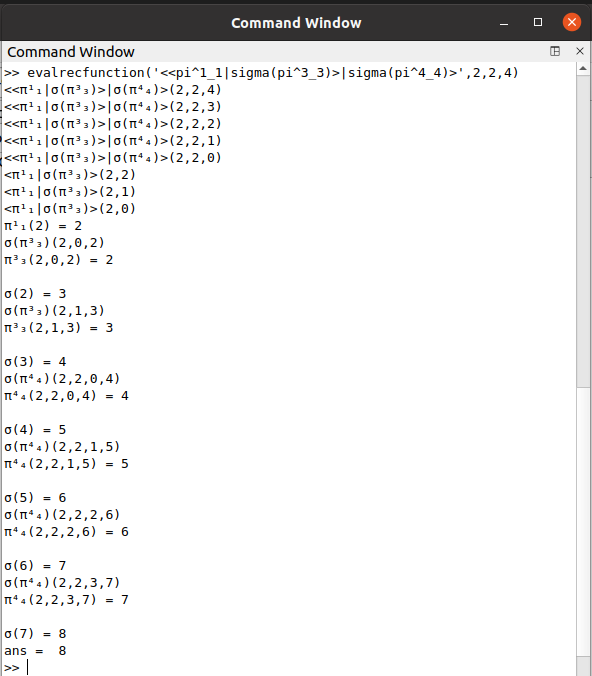
\includegraphics[width=12cm, height=11cm] {P3_E2.png}
    
\end{center}



\begin{center}
\end{center}
\section {Implement a WHILE program that computes the sum of three values. You must use an auxiliary variable that accumulates the result of the sum.}


\begin{algorithmic}

\While{X1!=0 }
\While{X2!=0 }
	\\\hspace{1cm}x3:=x3+1;
	\\\hspace{1cm}x2:=x2-1;\hspace{1cm}
\EndWhile
\vspace{0.15cm}
\\\hspace{0.5cm}x3:=x3+1;
\\\hspace{0.5cm}x1:=x1-1;
\vspace{0.15cm}
\EndWhile

\end{algorithmic}


\end{document}
